\documentclass{../../templates/amendment}
\usepackage{blindtext}
\usepackage[ngerman]{babel}
\usepackage{graphicx}
\usepackage{subcaption}
\usepackage[skip=2pt,font=small]{caption}

% \usepackage{showframe}
\occasion[Berzirksvertretung]{Bezirksvertretung Innenstadt-Ost}
\date{10. November 2020}
\begin{document}

\begin{boxed}{Calisthenics-Sportanlage Düsterstraße}{Jan Lucas Brause, Maximilian Sackel}

    Die Spiel- und Freizeitanlage an der Düsterstraße bildet einen Treffpunkt
    für alle Generationen und einen Querschnitt der Bevölkerung.
    Neben spielenden Kindern an den Spielgeräten und Jugendlichen auf den Bolzplatz
    finden sich dort genauso Eltern, die ihre Zeit am Calisthenics Park zum
    trainieren neben der Betreuung ihrer Kinder nutzen.
    Ebenso wird die Sportanlage von vielen Studierenden und jungen Berufstätigen als
    unverbindliche Trainingsmöglichkeit gut angenommen.

    Das Angebot ist jedoch auf die Sommermonate limitiert, da bei frühem Einbruch der
    Dunkelheit sowohl der Bolzplatz, Spielplatz und die Trainingsanlage nicht
    beleuchtet werden.
    Durch die fehlende Beleuchtung des Spiel- und Trainingsplatzes, ist eine Einsicht
    von Seiten der Straße nicht möglich.
    Dies hat zur Folge, dass der Platz vor allem in den Abendstunden als Rückzugsort
    zum Cannabiskonsum genutzt wird und ein "Angstraum" entsteht.

    Eine Beleuchtung mit Zeitschaltuhr verlängert die Nutzungsdauer und sorgt durch
    die Anwesenheit von Trainierenden sowie Eltern dafür, dass die Fläche unattraktiver für
    illegale Tätigkeiten wird.
    Des Weiteren existiert dadurch ein ausgeweitetes Sportangebot für finanziell
    eingeschränkte Bürger.

    Durch die gezielte Umpositionierung der bestehenden Mülleimer könnte zusätzlich die
    Verschmutzung der Spiel- und Sportflächen verringert werden.
    Sinnvoll wäre es die Mülleimer entsprechend der Nutzungspunkte aufzustellen
    und nicht dort, wo sie einfach zu montieren waren.

    Eine Erweiterung des bestehenden Wasserspielplatzes durch einen Trinkwasserspender,
    kommt sowohl den Kindern und Eltern als auch den Sportlern besonders in den
    Sommermonaten zugute.
    Da bereits Zuleitungen und Wasserinstallation vorhanden sind und gewartet
    werden, kann dies wahrscheinlich mit einem vergleichsweise geringen Aufwand
    umgesetzt werden.

    Im Anhang sind Abbildungen für eine bessere Einsicht der Sachlage
    angefügt.
    Einen Ortstermin zu einer Machbarkeitsstudie, sowie Verbesserung der Idee und
    Bündelung möglicherweise sinnvolle Sanierungen vorschläge, halten wir für sinnvoll.

    Über eine Bearbeitung und positive Rückmeldung würden wir uns sehr freuen.
    Selbstverständlich stehen wir gerne für Rückfragen jederzeit zur Verfügung.

    \begin{figure}[htpb]
        \centering
        \begin{subfigure}[]{0.49\textwidth}
            \begin{center}
                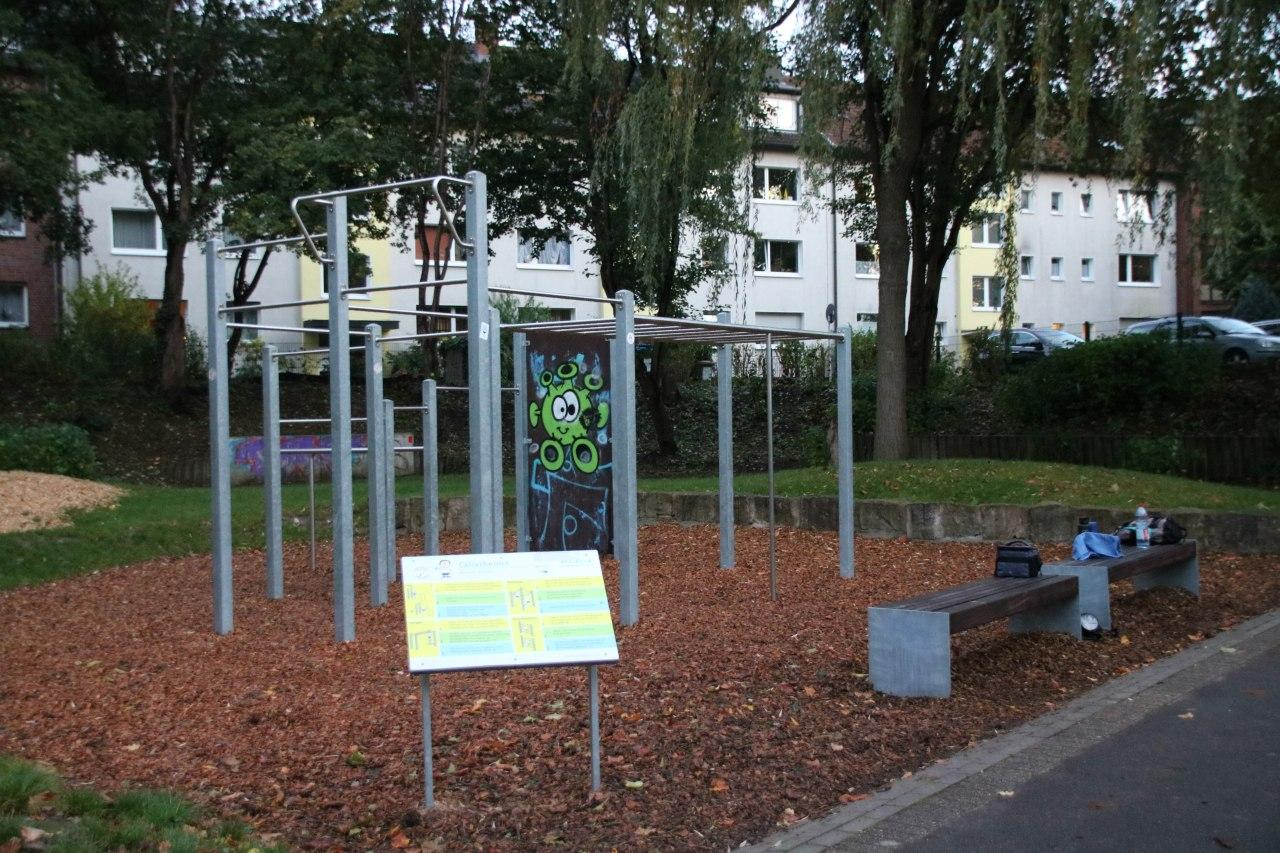
\includegraphics[width=\linewidth]{pictures/photo1.jpg}
                \caption{Calisthenics-Anlage}%
            \end{center}
        \end{subfigure}
        \begin{subfigure}[]{0.49\textwidth}
            \begin{center}
                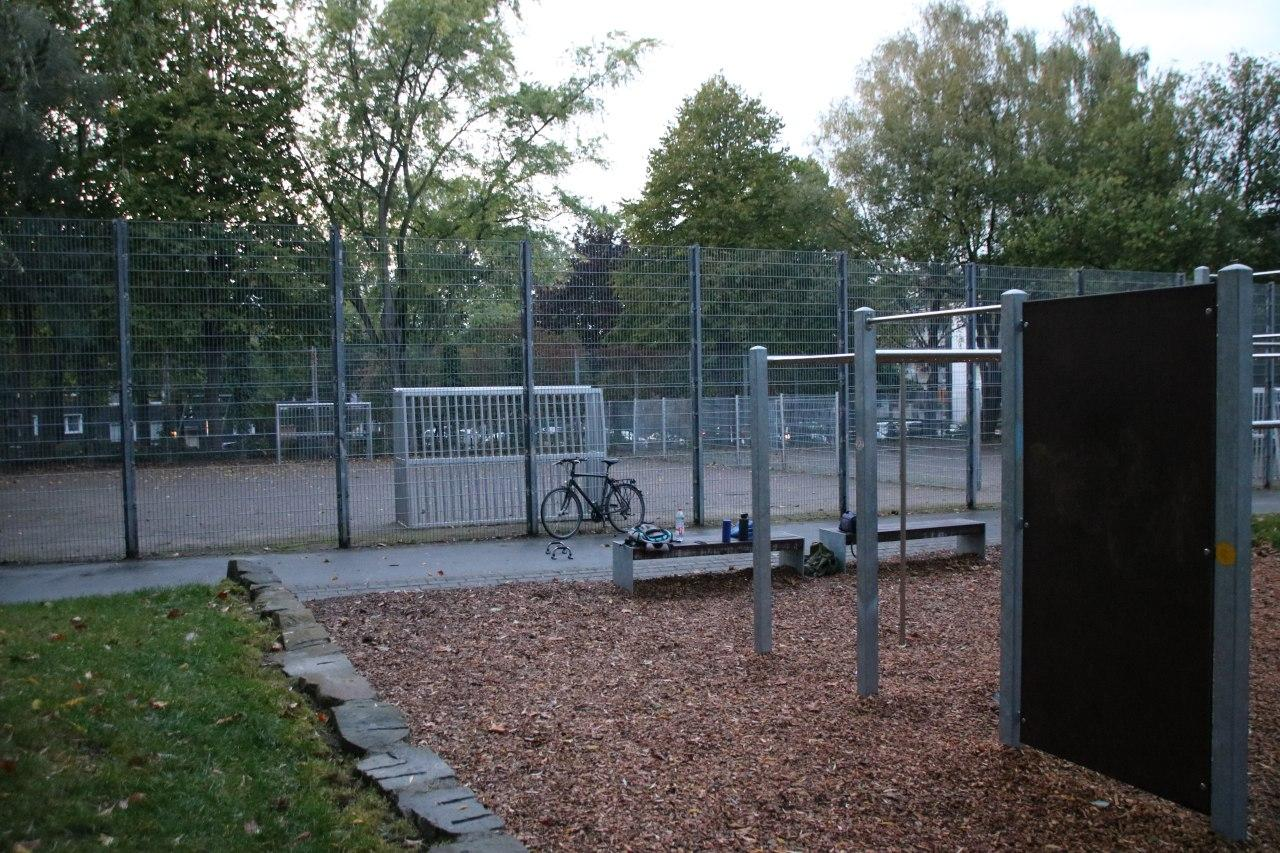
\includegraphics[width=\linewidth]{pictures/photo3.jpg}
                \caption{Angrenzender Boltzplatz}%
            \end{center}
        \end{subfigure}
        \caption{Verbesserungsbedürftige Ausleuchtungssituation begrenzt die
            Nutzungsdauer in den Wintermonaten und schafft durch schlechte Einsicht
            einen Angstraum.}
    \end{figure}

    \begin{figure}[htpb]
        \centering
        \begin{subfigure}[]{0.49\textwidth}
            \begin{center}
                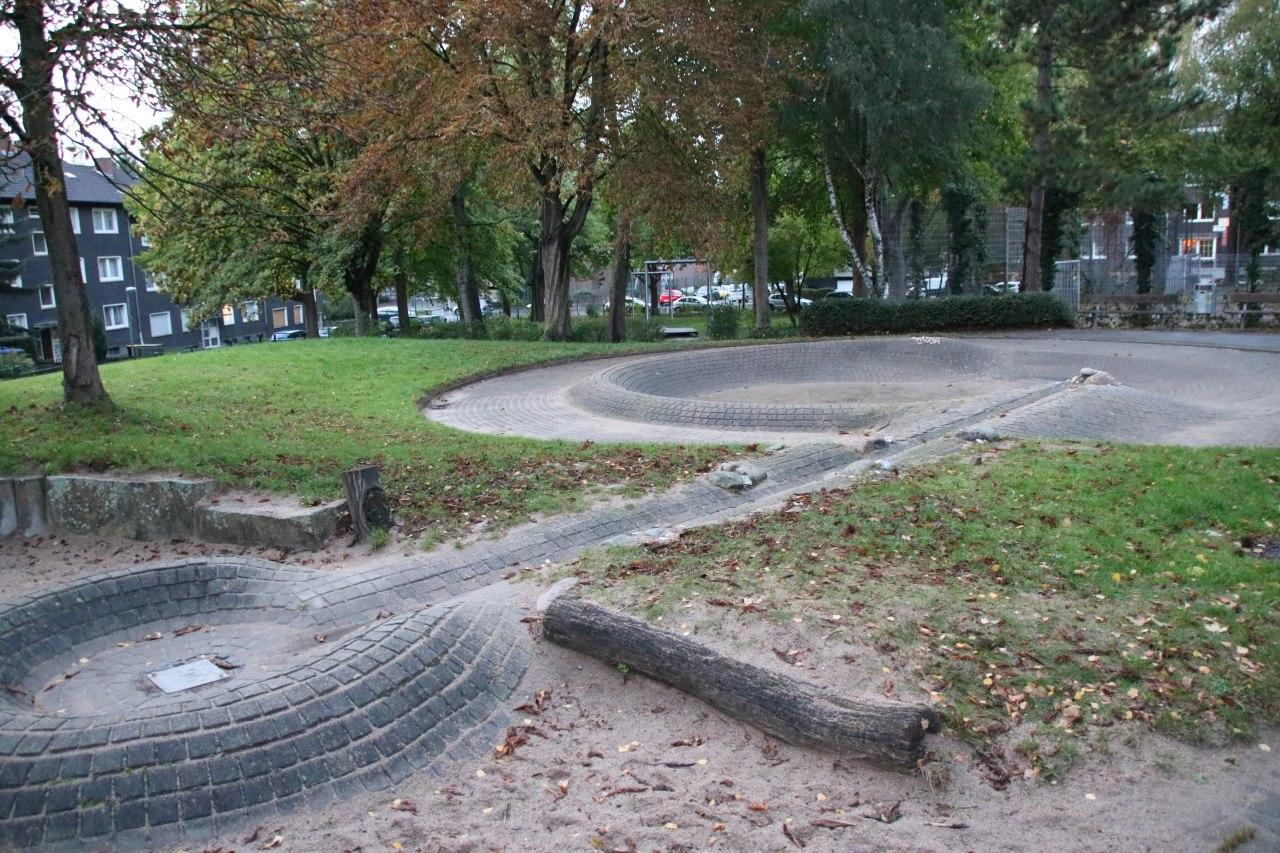
\includegraphics[width=\linewidth]{pictures/photo2.jpg}
                \caption{Wasserspielplatz}%
            \end{center}
        \end{subfigure}
        \begin{subfigure}[]{0.49\textwidth}
            \begin{center}
                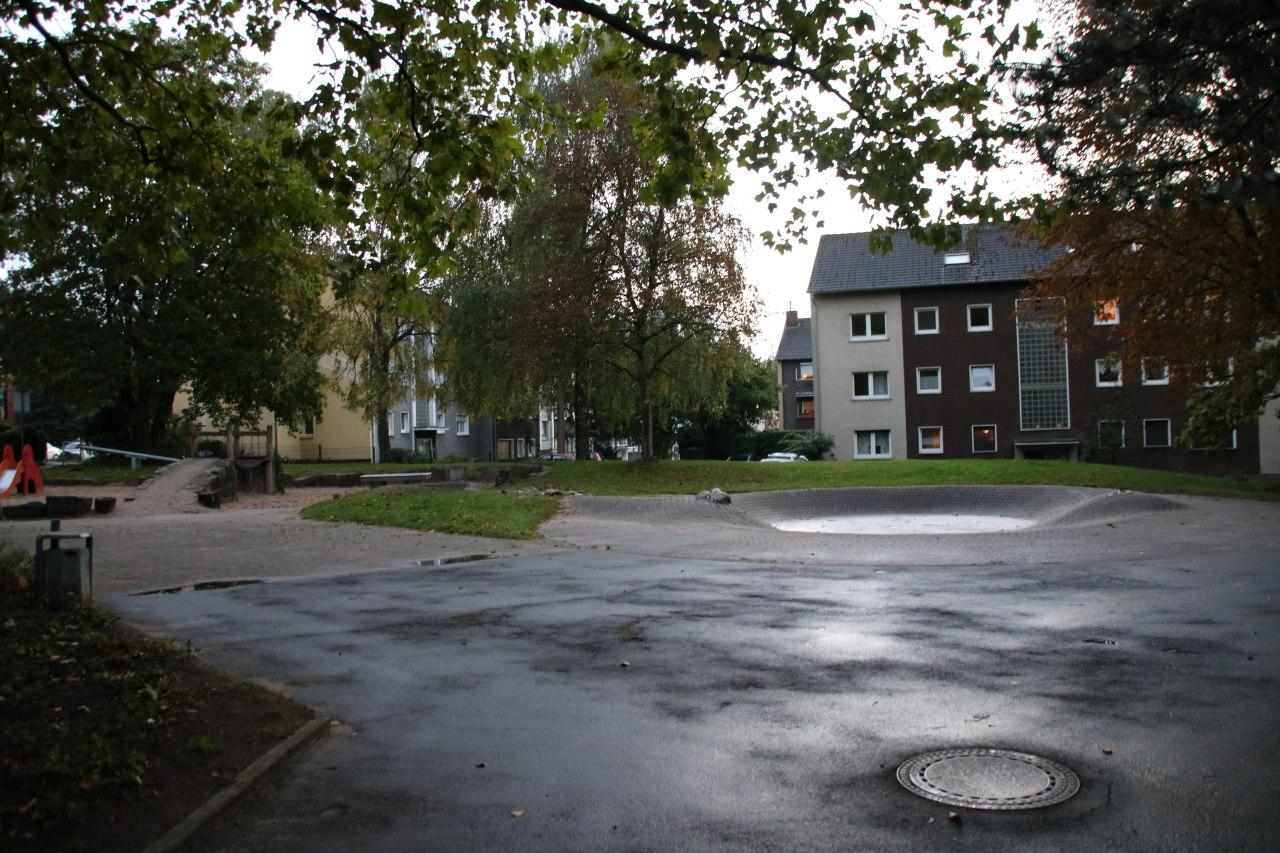
\includegraphics[width=\linewidth]{pictures/photo4.jpg}
                \caption{ungenutzte Fläche}%
            \end{center}
        \end{subfigure}
        \caption{Erweiterung des bestehenden Wasserspielplatzes durch einen
                 Brunnen, würde die Trinkwasserversorgung für spielende Kinder, Eltern 
                 sowie Trainierende sicherstellen.}
    \end{figure}
\end{boxed}

\end{document}
